\section{سوال دوم}
در این بخش هواپیمای بوئینگ 747 مورد بررسی قرار گرفته است.
 \begin{figure}[H]
	\centering
	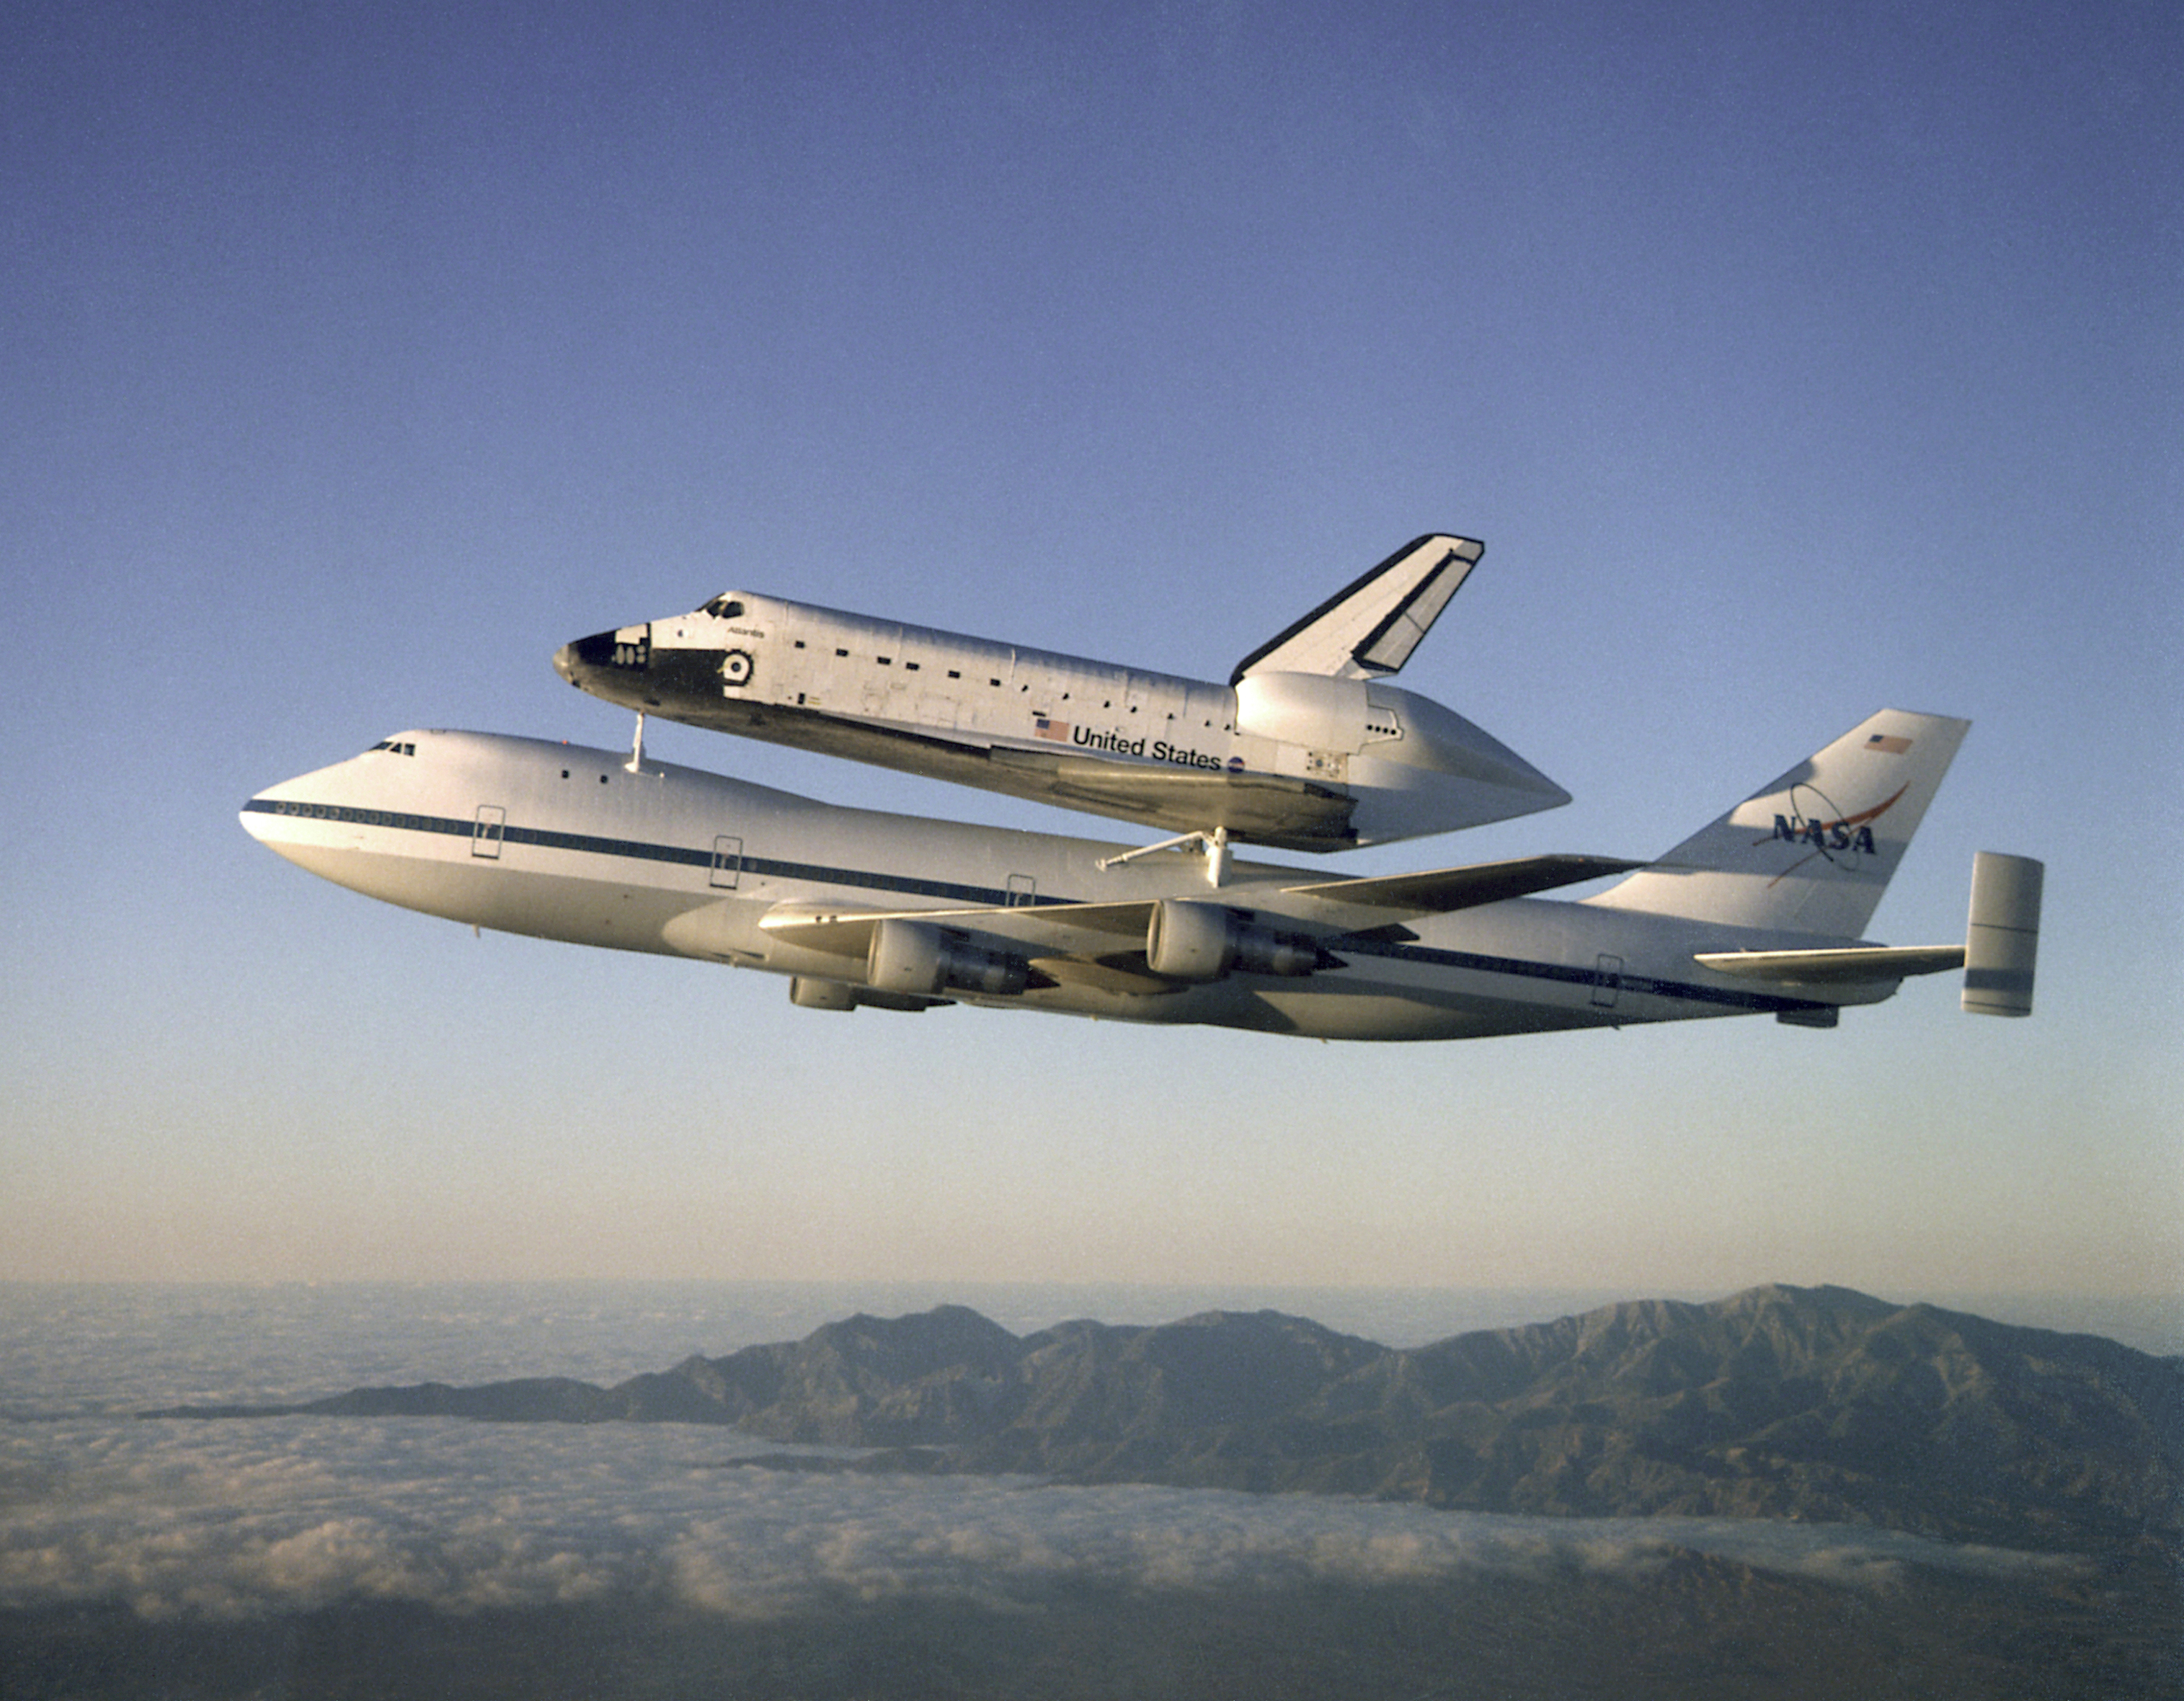
\includegraphics[width=\linewidth]{../Figure/Q2/Atlantis_on_Shuttle_Carrier_Aircraft.jpg}
	\caption{بوئینگ ۷۴۷ در حال حمل شاتل
	}
\end{figure}
\subsection{بخش اول}
در هواپیماهای ترابری به طور معمول از سیستم ناوبری ترکیبی اینرسی و رادیویی استفاده می‌شود. در فاز پرواز مستقیم، سیستم هدایت به‌صورت اینرسی و در هنگام فرود، ترکیب اینرسی و پرتوسوار است.

\subsection{بخش دوم}
در این بخش مدل سیمولینک هدایت و ناوبری آورده شده است. در این سیمولینک زیرسیستم‌ها نیز در نظر گرفته شده‌اند.
 \begin{figure}[H]
	\centering
	\includegraphics[width=\linewidth]{../Figure/Q2/Q2_simulink.pdf}
	\caption{مدل هدایت و ناوبری در محیط سیمولینک
	}
\end{figure}

